%% -*- Mode:LaTeX -*-

\chapterpreamble{0.6\textwidth}{Ingmar Bergman}{%
  Before, fortunately, I am by nature an autodidact, one who can teach himself---though it's an
  uncomfortable thing at times. Self-taught people sometimes cling too much to the technical side,
  the sure side and place technical perfection too high.
}

\chapter{How to \ldots}
\label{app:how-to}

\section{Write a Technical Text}
\label{app:how-to:write+a+technical+text}

\begin{itemize}
\item \citetitle{Booth:CR:2008} \autocite{Booth:CR:2008}
\end{itemize}
\par

\section{Citations}
\label{app:how-to:citations}

Single author:
\begin{itemize}
\item \verb!\autocite{Nicodemus:DREOS:1965}!: \autocite{Nicodemus:DREOS:1965}
\item \verb!\citetitle{Nicodemus:DREOS:1965}!: \citetitle{Nicodemus:DREOS:1965}
\item \verb!\citeauthor{Nicodemus:DREOS:1965}!: \citeauthor{Nicodemus:DREOS:1965}
\item \verb!\citeyear{Nicodemus:DREOS:1965}!: \citeyear{Nicodemus:DREOS:1965}
\end{itemize}
Multiple authors:
\begin{itemize}
\item \verb!\autocite{Sutherland:CTHSA:1974}!: \autocite{Sutherland:CTHSA:1974}
\item \verb!\citetitle{Sutherland:CTHSA:1974}!: \citetitle{Sutherland:CTHSA:1974}
\item \verb!\citeauthor{Sutherland:CTHSA:1974}!: \citeauthor{Sutherland:CTHSA:1974}
\item \verb!\citeyear{Sutherland:CTHSA:1974}!: \citeyear{Sutherland:CTHSA:1974}
\end{itemize}
\par

\section{Figures}
\label{app:how-to:figures}

\begin{figure}
  \centering
  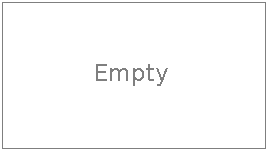
\includegraphics[draft=false,width=0.75\linewidth]{figures/empty_lscape}
  \caption[A single landscape figure]{A single landscape figure.}
  \label{fig:how-to:figures:lscape}
\end{figure}
Figure~\ref{fig:how-to:figures:lscape} contains a single image in landscape format scaled to 75\% of
the current line width.
\begin{figure}
  \centering
  \subfloat[][]{%
    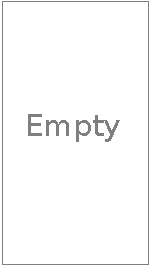
\includegraphics[draft=false,width=0.375\linewidth]{figures/empty_portrait}
    \label{fig:how-to:figures:portait:a}
  }
  \subfloat[][]{%
    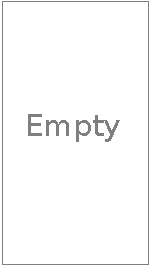
\includegraphics[draft=false,width=0.375\linewidth]{figures/empty_portrait}
    \label{fig:how-to:figures:portait:b}
  }
  \caption[A single portrait figure]{A single figure containing sub-figures
    (\protect\subref{fig:how-to:figures:portait:a} and
    \protect\subref{fig:how-to:figures:portait:b})\@.}
  \label{fig:how-to:figures:portait}
\end{figure}
Figures~\ref{fig:how-to:figures:portait:a} and \ref{fig:how-to:figures:portait:b} are sub-figures
withing figure~\ref{fig:how-to:figures:portait} but can be individually referred
to. Figures~\ref{fig:how-to:figures:portait:a} and \ref{fig:how-to:figures:portait:b} are both
scaled to 37.5\% of the current line width.
\par

\section{Tables}
\label{app:how-to:tables}

\begin{table}
  \centering
  \sffamily
  \begin{tabular}{lccr}
    \toprule
    Left aligned  & Centered & Centered & Right aligned\\
    \midrule
    \ldots & \ldots   & \ldots   & \ldots \\
    \ldots & \ldots   & \ldots   & \ldots \\
    \ldots & \ldots   & \ldots   & \ldots \\
    \ldots & \ldots   & \ldots   & \ldots \\
    \ldots & \ldots   & \ldots   & \ldots \\
    \bottomrule
  \end{tabular}
  \caption[A simple table]{A simple table.}
  \label{tab:how-to:tables:example1}
\end{table}
\begin{table}
  \centering
  \sffamily
  \rowcolors{2}{}{gray!10}
  \begin{tabular}{lcccr}
    \toprule
    Left aligned  & Centered & Centered & Centered & Right aligned\\
    \midrule
    \ldots & \ldots   & \ldots   & \ldots   & \ldots \\
    \ldots & \ldots   & \ldots   & \ldots   & \ldots \\
    \ldots & \ldots   & \ldots   & \ldots   & \ldots \\
    \ldots & \ldots   & \ldots   & \ldots   & \ldots \\
    \ldots & \ldots   & \ldots   & \ldots   & \ldots \\
    \bottomrule
  \end{tabular}
  \caption[Alternating row-color table]{A table with alternating row colors.}
  \label{tab:how-to:tables:example2}
\end{table}
\ldots
\par

\section{Miscellaneous}
\label{app:how-to:miscellaneous}

\ldots
\par

%%% Local Variables:
%%% mode: latex
%%% TeX-master: "../main"
%%% End:
